\section{Introduction}
In recent years, deep learning has emerged as a powerful tool for solving complex problems that were considered to be difficult in the
past. It has brought a step change in the machine's ability to solve tasks like object recognition~\cite{donahue14,he2016deep}, facial
recognition~\cite{parkhi2015deep,sun2014deep}, speech processing~\cite{pmlrv48amodei16}, and machine translation~\cite{bahdanau2014neural}.
While many of these tasks are also important on mobiles and the Internet of Things (IoT), existing solutions are often
computation-intensive and require a large amount of resources for the model to operate. As a result, performing deep
inference\footnote{Inference in this paper refers to apply a pre-trained model on an input to obtain the corresponding output. This is
different from statistical inference.} on embedded devices can lead to long runtime and the consumption of abundant amounts of resources,
including CPU, memory, and power, even for simple tasks~\cite{CanzianiPC16}. Without a solution,
 the hoped-for advances on embedded sensing will not arrive.


Numerous approaches have been proposed to accelerate deep inference on embedded devices. These include designing purpose-built hardware to
reduce the computation or memory latency~\cite{georgiev2017low}, compressing a pre-trained model to reduce its storage and memory footprint
as well as computational requirements~\cite{han2016eie}, and offloading some, or all, computation to a cloud
server~\cite{Kang2017neurosurgeon,teerapittayanon2017distributed}. Compared to specialized hardware, model compression techniques have the
advantage of being readily deployable on commercial-off-the-self hardware; and compared to computation offloading, compression enables
local, on-device inference which in turn reduces the response latency and has fewer privacy concerns. Such advantages make model
compressions attractive on resource-constrained IoT devices where computation offloading is infeasible.


However, model compression is not a free lunch as it comes at the cost of loss in prediction accuracy~\cite{Cheng2017A}. This means that
one must carefully choose the model compression technique and its parameters to effectively trade precision for time, energy, as well as
computation and resource requirements. Furthermore, as we will show in this paper, the reduction in the model size does not necessarily
translate into faster inference time. Because there is no guarantee for a compression technique to be beneficial, we need to know when and
how to apply a compression technique.

Our work aims to characterize deep learning model compression techniques for embedded inference. Knowing this not only informs the better
deployment of computation-intensive models, but also enables designing more efficient architectures for deep learning models and embedded
hardware.

To that end, we develop a quantitative approach  to characterize two mainstream model compression techniques, pruning~\cite{Cheng2017A} and
data quantization~\cite{Gong2014Compressing}. We apply the techniques to the image classification and the natural language processing (NLP)
domains, two areas where deep learning has made great breakthroughs and a rich set of pre-trained models are available. We evaluate the
compression results on the NVIDIA Jetson TX2 embedded deep learning platform and consider a wide range of influential deep learning models.
We use the 50K images from the ImageNet ILSVRC 2012 validation dataset~\cite{imagenet2012} for image classification and a corpus of ten
thousands text samples~\cite{acl2016} for NLP.


We show that while there is significant gain for choosing the right compression technique and parameters, mistakes can seriously hurt the
performance. We then quantify how different model compression techniques and parameters affect the inference time, energy consumption,
model storage requirement and prediction accuracy. As a result, our work provides insights on when and how to apply deep learning model
compression techniques on embedded devices, as well as guidelines on designing schemes to adapt deep learning model optimisations for
various application constraints.

\begin{figure*}[!t]
\centering
\subfloat[][Model size]{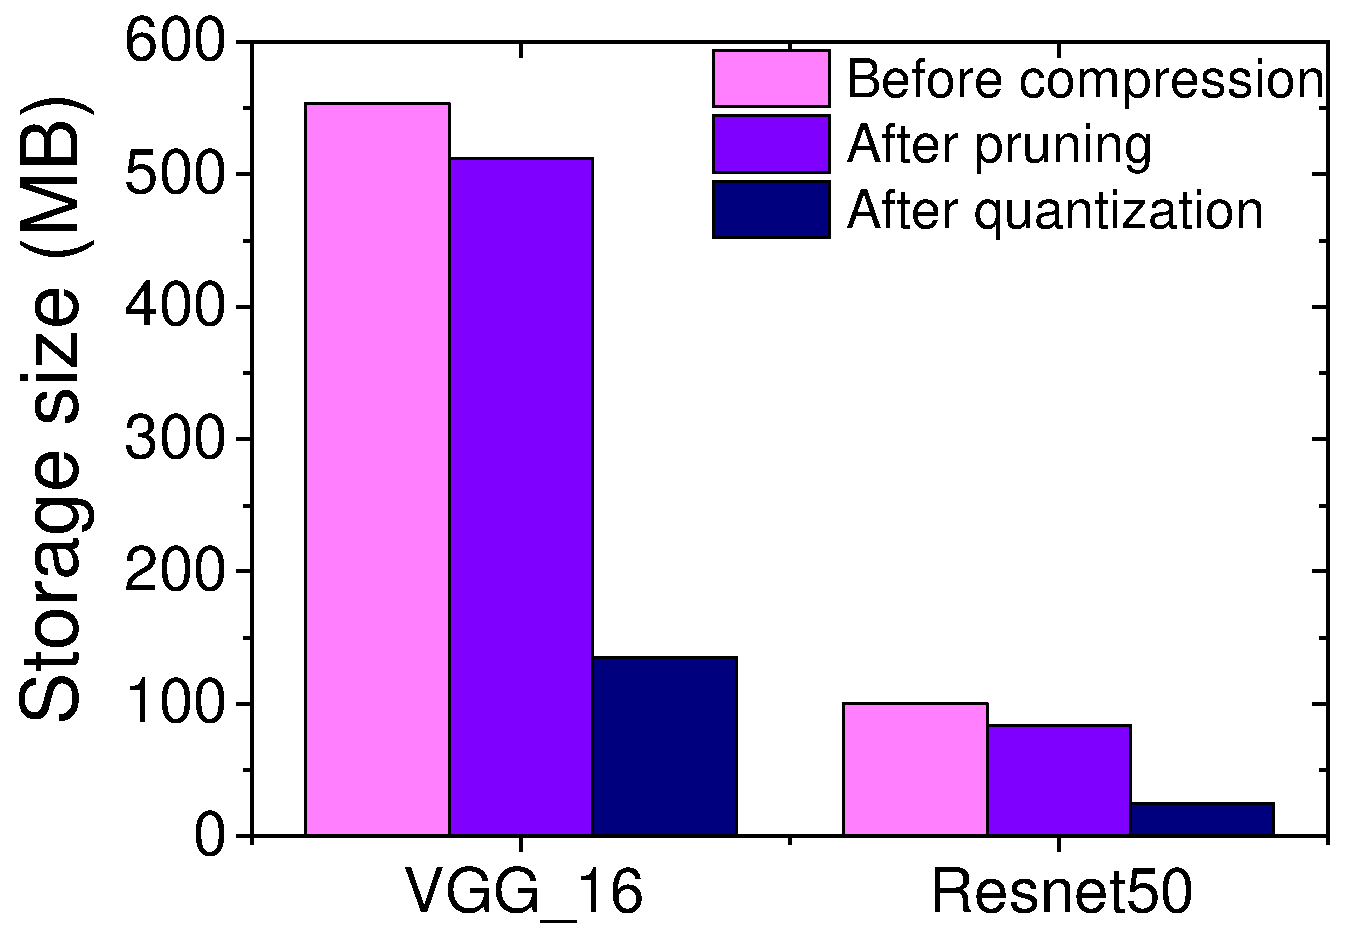
\includegraphics[width=0.24\textwidth]{figure/motivation_size1.pdf}}
\hfill
\subfloat[][Inference time]{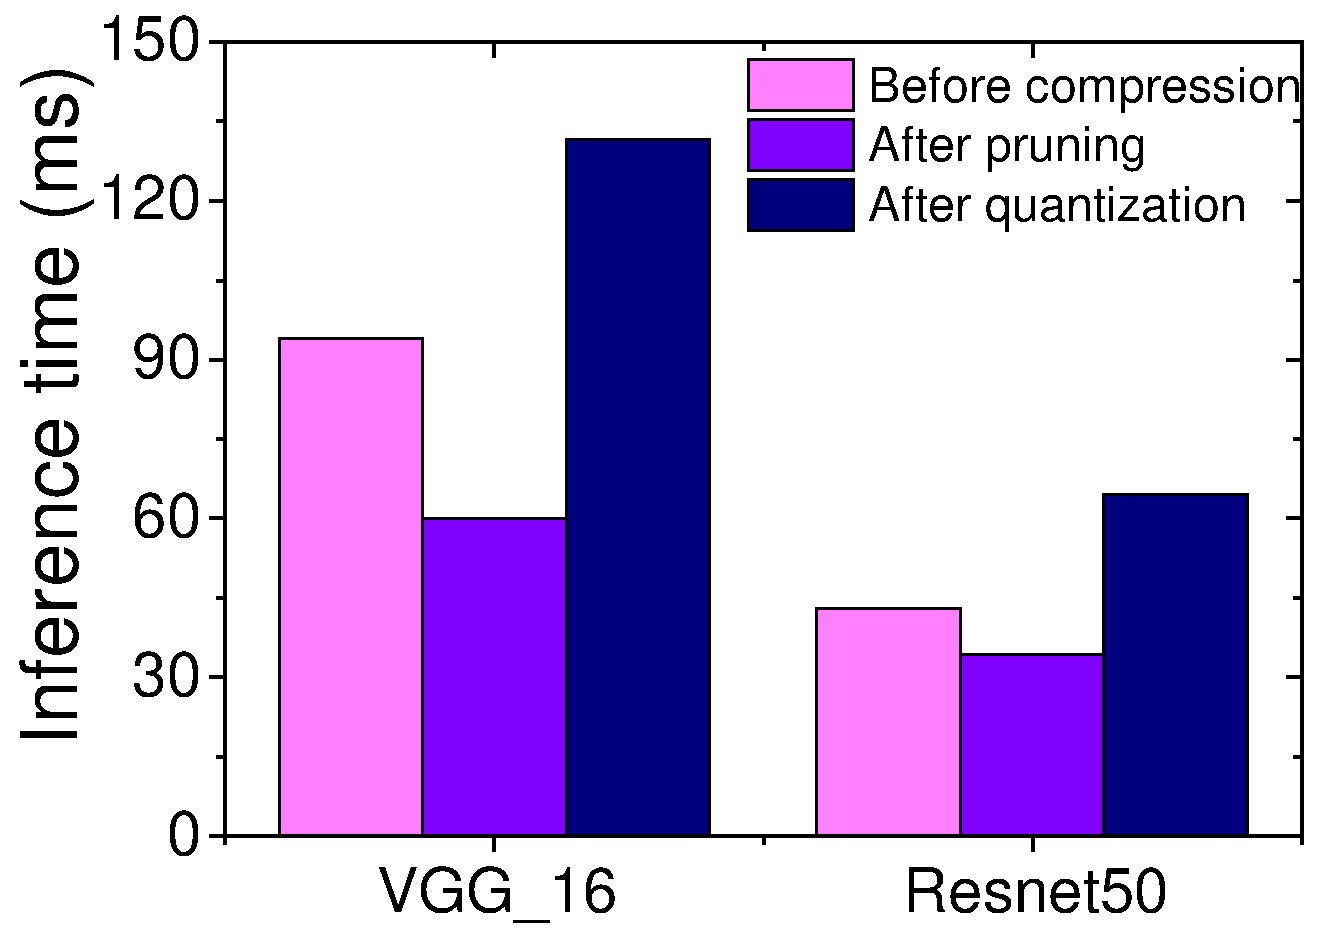
\includegraphics[width=0.24\textwidth]{figure/motivation_time1.pdf}}
\hfill
\subfloat[][Energy consunption]{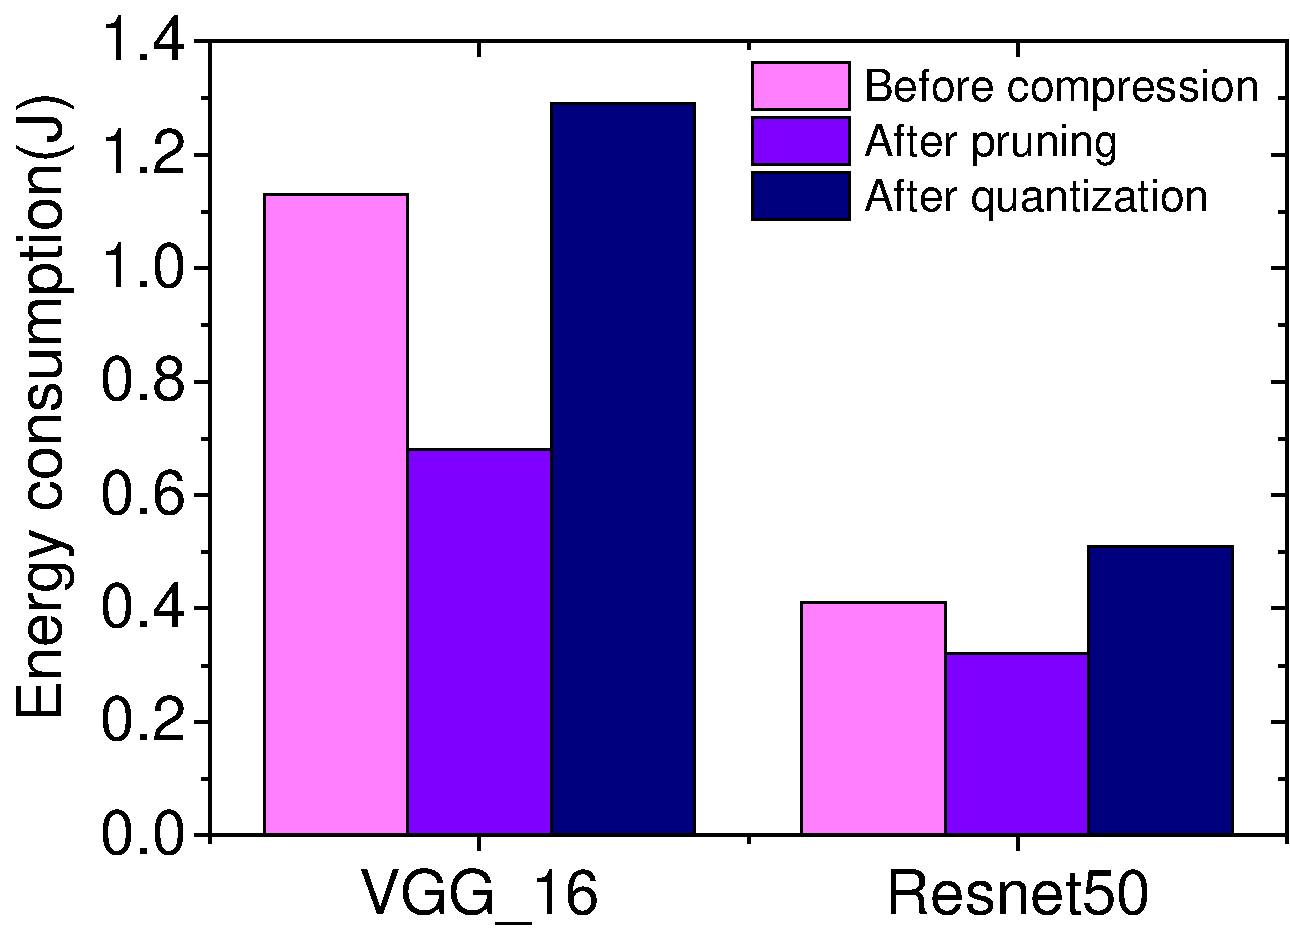
\includegraphics[width=0.23\textwidth]{figure/motivation_energy1.pdf}}
\hfill
\subfloat[][Accuracy]{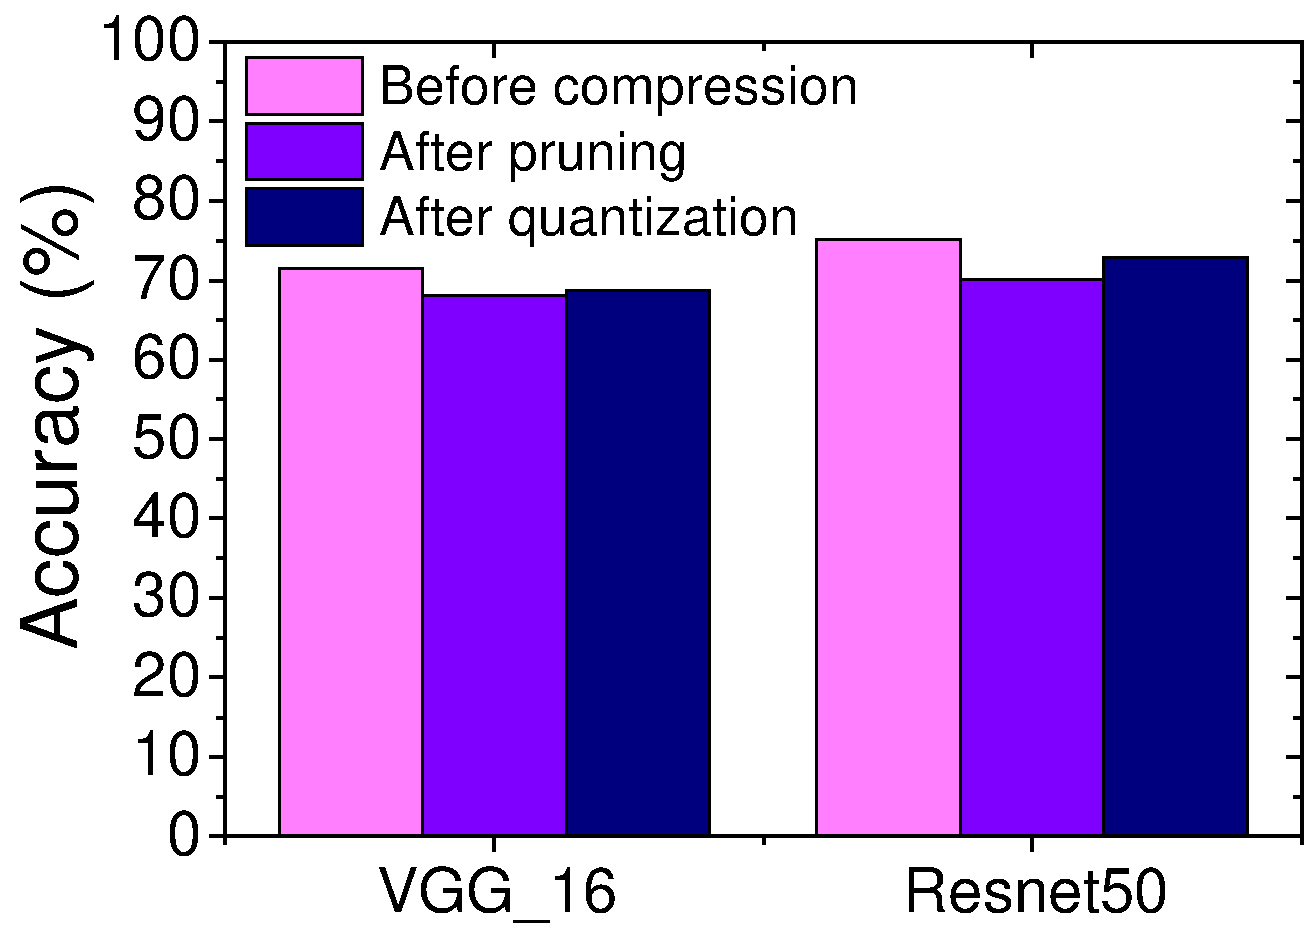
\includegraphics[width=0.24\textwidth]{figure/motivation_accuracy1.pdf}}
\hfill
\caption{The achieved model size (a) inference time (b) energy consumption (c) and accuracy (d) before and after the compression by \quantization and \pruning.
The compression technique to use depends on the optimization target.}
\vspace{-4mm}
\label{fig:motivation}
\end{figure*}


The main contributions of this paper are two folds:

\begin{itemize}
\item We present an extensive study to characterize and understand how two popular model compression techniques perform on a
    representative embedded deep learning platform and a wide range of deep neural network architectures;
\item Our work offers insights on when and how to apply compression techniques for embedded deep inference.
\end{itemize}

We believe there is an opportunity to enable for performing efficient deep inference locally on the device. We thus hope the empirical
evidences in the paper can provide the stepping stones and encourage research on this promising direction.
